\documentclass[11pt,letterpaper]{article}
\usepackage[utf8]{inputenc}
\usepackage[T1]{fontenc}
\usepackage[spanish]{babel}
\usepackage{amsmath}
\usepackage{amsfonts}
\usepackage{amssymb}
\usepackage{graphicx}
\usepackage{lmodern}
\usepackage{xspace}
\usepackage{multicol}
\usepackage{hyperref}
\usepackage{float}
\usepackage{hyperref}
\usepackage{color}
\usepackage{framed}
\usepackage[thinc]{esdiff}	
\DeclareUnicodeCharacter{2212}{-}
\usepackage{biblatex}
\addbibresource{biblio.bib}

\DeclareUnicodeCharacter{0301}{\'{i}}
\usepackage{enumerate}% http://ctan.org/pkg/enumerate

\usepackage[left=2cm,right=2cm,top=2cm,bottom=2cm]{geometry}

\newcommand{\X}{\mathbb{X}}
\newcommand{\x}{\mathbf{x}}
\newcommand{\Y}{\mathbf{Y}}
\newcommand{\y}{\mathbf{y}}
\newcommand{\xbarn}{\bar{x}_n}
\newcommand{\ybarn}{\bar{y}_n}
\newcommand{\paren}[1]{\left( #1 \right)}
\newcommand{\llaves}[1]{\left\lbrace #1 \right\rbrace}
\newcommand{\barra}{\,\vert\,}
\newcommand{\mP}{\mathbb{P}}
\newcommand{\mE}{\mathbb{E}}
\newcommand{\mR}{\mathbb{R}}
\newcommand{\mJ}{\mathbf{J}}
\newcommand{\mX}{\mathbf{X}}
\newcommand{\mS}{\mathbf{S}}
\newcommand{\mA}{\mathbf{A}}
\newcommand{\unos}{\boldsymbol{1}}
\newcommand{\xbarnv}{\bar{\mathbf{x}}_n}
\newcommand{\abs}[1]{\left\vert #1 \right\vert}
\newcommand{\muv}{\boldsymbol{\mu}}
\newcommand{\mcov}{\boldsymbol{\Sigma}}
\newcommand{\vbet}{\boldsymbol{\beta}}
\newcommand{\veps}{\boldsymbol{\epsilon}}
\newcommand{\mcC}{\mathcal{C}}
\newcommand{\mcR}{\mathcal{R}}
\newcommand{\mcN}{\mathcal{N}}

\newcommand{\ceros}{\boldsymbol{0}}
\newcommand{\mH}{\mathbf{H}}
\newcommand{\ve}{\mathbf{e}}
\newcommand{\avec}{\mathbf{a}}
\newcommand{\res}{\textbf{RESPUESTA}\\}

\newcommand{\defi}[3]{\textbf{Definición:#3}}
\newcommand{\fin}{$\blacksquare.$}
\newcommand{\finf}{\blacksquare.}
\newcommand{\tr}{\text{tr}}
\newcommand*{\temp}{\multicolumn{1}{r|}{}}
\newtheorem{ej}{Ejemplo}[section]
\newcommand{\grstep}[2][\relax]{%
   \ensuremath{\mathrel{
       {\mathop{\longrightarrow}\limits^{#2\mathstrut}_{
                                     \begin{subarray}{l} #1 \end{subarray}}}}}}
\newcommand{\swap}{\leftrightarrow}



\newcommand{\gen}{\text{gen}}
\newtheorem{thmt}{Teorema:}
\newtheorem{thmd}{Definición:}
\newtheorem{thml}{Lema:}
\newtheorem{thme}{Ejemplo:}

% New command master
\newcommand{\nns}{\textit{neural networks}}
\newcommand{\da}{\textit{data augentation}}
\newcommand{\AA}{\textit{AutoAugment}}

\title{Anteproyecto de reporte de tesis de maestría}
\author{Enrique Santibáñez Cortés,
\textit{Asesor de tesis:} Dr. Alejandro Rosales}
\begin{document}
\maketitle

\section*{Planteamiento del problema, definición del problema}
En este trabajo se desarrollara el plantamiento del trabajo de tesis para obtener el grado de Maestro en Computo Estadístico.

En este tema, la idea es desarrollar un método de AutoML para escoger la
estrategia de aumento de datos e hiper-parámetros del modelo que maximice una medida 


\section*{Antecedentes y justificación}
Tenemos que 
Las \nns son propensas a \textit{overfit} cuando el conjunto de datos es limitado. \textit{Data Augmentation} sirve como un tipo de regularización para el entrenamiento de las \nns, y en la mayoría de las veces reduce el \textit{overfitting}. \cite{augmented_random_search} \textit{AutoAugment} es una propuesta de búsqueda automática para el mejor enfoque de \ad que pueda incorporar invarianza y generalizar bien a través de diferentes modelos y conjuntos de datos. Debido a como se realiza la busqueda en un espacio discreto, \textit{AutoAugment} puede encontrar algunas sub-políticas es decir, encuentra una solución sub-óptima.\\

\cite{learning_data_augmentation_2} Aunque \da ha demostrado mejorar significativamente la clasificación de imágenes no se ha investigado a fondo su potencial para la detección de objetos. Por lo cuál, en este estudio presentan el impacto de \da en la detección de objetos. En el dominio de las imágenes comúnmente el aumento incluye traslación de imágenes, rotación, y los clasificadores más modernos usan estrategias \da implementadas a mano. En comparación con la clasificación de imágenes, desarrollar una estrategia de \da para la detección de objetos es más difícil porque hay más formas y complejidades introducidas al distorsionar la imagen, las ubicaciones de los cuadros delimitadores y los tamaños de los objetos en los conjuntos de datos de detección. \\

\cite{populaion_based_augmentatio_3} En este articulo se centra en obtener una metodología más eficiente (en tiempo computacional) comparado con el estado del arte en el problema de clasificación de imágenes. Su enfoque fue inspirado en el trabajo de optimización de hiperparametros. Existen muchos trabajos previos para obtener buenos hiperparametros, específicamente en Optimización Bayesiana. 


Los enfoques actuales del estado del arte como \AA son computacionalmente ineficientes para ejecutarse para un usuario común. En los últimos años se ha propuestos diferentes variaciones de \AA, como por ejemplo: \textit{Population Based Augmentation} (PBA) \cite{populaion_based_augmentatio_3}, \\


Unos de los primeros enfoques para encontrar la mejor política de \ad es formulando un problema de búsqueda discreta.  
\begin{figure}[H]
    \centering
    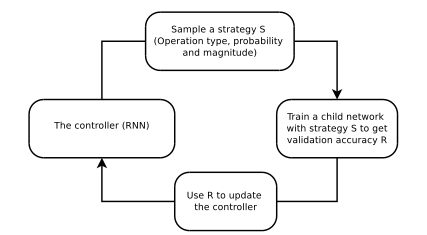
\includegraphics[scale=0.5]{figure/enfoque_AutoAugment.png}
    \caption{Framework AutoAugment \cite{cubuk_autoaugment_4}}
    \label{fig:enfoque_AutoAugment}
\end{figure}


\section*{Objetivos}



\section*{Metodología}

\section*{Bibliografía}





\printbibliography

\end{document}